% Options for packages loaded elsewhere
\PassOptionsToPackage{unicode}{hyperref}
\PassOptionsToPackage{hyphens}{url}
%
\documentclass[
  11pt,
]{article}
\usepackage{amsmath,amssymb}
\usepackage{lmodern}
\usepackage{setspace}
\usepackage{iftex}
\ifPDFTeX
  \usepackage[T1]{fontenc}
  \usepackage[utf8]{inputenc}
  \usepackage{textcomp} % provide euro and other symbols
\else % if luatex or xetex
  \usepackage{unicode-math}
  \defaultfontfeatures{Scale=MatchLowercase}
  \defaultfontfeatures[\rmfamily]{Ligatures=TeX,Scale=1}
  \setmainfont[]{TeX Gyre Termes}
  \setmonofont[]{DejaVu Sans Mono}
\fi
% Use upquote if available, for straight quotes in verbatim environments
\IfFileExists{upquote.sty}{\usepackage{upquote}}{}
\IfFileExists{microtype.sty}{% use microtype if available
  \usepackage[]{microtype}
  \UseMicrotypeSet[protrusion]{basicmath} % disable protrusion for tt fonts
}{}
\makeatletter
\@ifundefined{KOMAClassName}{% if non-KOMA class
  \IfFileExists{parskip.sty}{%
    \usepackage{parskip}
  }{% else
    \setlength{\parindent}{0pt}
    \setlength{\parskip}{6pt plus 2pt minus 1pt}}
}{% if KOMA class
  \KOMAoptions{parskip=half}}
\makeatother
\usepackage{xcolor}
\IfFileExists{xurl.sty}{\usepackage{xurl}}{} % add URL line breaks if available
\IfFileExists{bookmark.sty}{\usepackage{bookmark}}{\usepackage{hyperref}}
\hypersetup{
  pdftitle={Files All the Way Down: A Design Space Analysis of Filesystem-Native LLM Tool Integration},
  pdfauthor={Natan Loterio},
  hidelinks,
  pdfcreator={LaTeX via pandoc}}
\urlstyle{same} % disable monospaced font for URLs
\usepackage[top=1in,bottom=1in,left=1.25in,right=1.25in]{geometry}
\usepackage{color}
\usepackage{fancyvrb}
\newcommand{\VerbBar}{|}
\newcommand{\VERB}{\Verb[commandchars=\\\{\}]}
\DefineVerbatimEnvironment{Highlighting}{Verbatim}{commandchars=\\\{\}}
% Add ',fontsize=\small' for more characters per line
\newenvironment{Shaded}{}{}
\newcommand{\AlertTok}[1]{\textcolor[rgb]{1.00,0.00,0.00}{\textbf{#1}}}
\newcommand{\AnnotationTok}[1]{\textcolor[rgb]{0.38,0.63,0.69}{\textbf{\textit{#1}}}}
\newcommand{\AttributeTok}[1]{\textcolor[rgb]{0.49,0.56,0.16}{#1}}
\newcommand{\BaseNTok}[1]{\textcolor[rgb]{0.25,0.63,0.44}{#1}}
\newcommand{\BuiltInTok}[1]{#1}
\newcommand{\CharTok}[1]{\textcolor[rgb]{0.25,0.44,0.63}{#1}}
\newcommand{\CommentTok}[1]{\textcolor[rgb]{0.38,0.63,0.69}{\textit{#1}}}
\newcommand{\CommentVarTok}[1]{\textcolor[rgb]{0.38,0.63,0.69}{\textbf{\textit{#1}}}}
\newcommand{\ConstantTok}[1]{\textcolor[rgb]{0.53,0.00,0.00}{#1}}
\newcommand{\ControlFlowTok}[1]{\textcolor[rgb]{0.00,0.44,0.13}{\textbf{#1}}}
\newcommand{\DataTypeTok}[1]{\textcolor[rgb]{0.56,0.13,0.00}{#1}}
\newcommand{\DecValTok}[1]{\textcolor[rgb]{0.25,0.63,0.44}{#1}}
\newcommand{\DocumentationTok}[1]{\textcolor[rgb]{0.73,0.13,0.13}{\textit{#1}}}
\newcommand{\ErrorTok}[1]{\textcolor[rgb]{1.00,0.00,0.00}{\textbf{#1}}}
\newcommand{\ExtensionTok}[1]{#1}
\newcommand{\FloatTok}[1]{\textcolor[rgb]{0.25,0.63,0.44}{#1}}
\newcommand{\FunctionTok}[1]{\textcolor[rgb]{0.02,0.16,0.49}{#1}}
\newcommand{\ImportTok}[1]{#1}
\newcommand{\InformationTok}[1]{\textcolor[rgb]{0.38,0.63,0.69}{\textbf{\textit{#1}}}}
\newcommand{\KeywordTok}[1]{\textcolor[rgb]{0.00,0.44,0.13}{\textbf{#1}}}
\newcommand{\NormalTok}[1]{#1}
\newcommand{\OperatorTok}[1]{\textcolor[rgb]{0.40,0.40,0.40}{#1}}
\newcommand{\OtherTok}[1]{\textcolor[rgb]{0.00,0.44,0.13}{#1}}
\newcommand{\PreprocessorTok}[1]{\textcolor[rgb]{0.74,0.48,0.00}{#1}}
\newcommand{\RegionMarkerTok}[1]{#1}
\newcommand{\SpecialCharTok}[1]{\textcolor[rgb]{0.25,0.44,0.63}{#1}}
\newcommand{\SpecialStringTok}[1]{\textcolor[rgb]{0.73,0.40,0.53}{#1}}
\newcommand{\StringTok}[1]{\textcolor[rgb]{0.25,0.44,0.63}{#1}}
\newcommand{\VariableTok}[1]{\textcolor[rgb]{0.10,0.09,0.49}{#1}}
\newcommand{\VerbatimStringTok}[1]{\textcolor[rgb]{0.25,0.44,0.63}{#1}}
\newcommand{\WarningTok}[1]{\textcolor[rgb]{0.38,0.63,0.69}{\textbf{\textit{#1}}}}
\usepackage{longtable,booktabs,array}
\usepackage{calc} % for calculating minipage widths
% Correct order of tables after \paragraph or \subparagraph
\usepackage{etoolbox}
\makeatletter
\patchcmd\longtable{\par}{\if@noskipsec\mbox{}\fi\par}{}{}
\makeatother
% Allow footnotes in longtable head/foot
\IfFileExists{footnotehyper.sty}{\usepackage{footnotehyper}}{\usepackage{footnote}}
\makesavenoteenv{longtable}
\usepackage{graphicx}
\makeatletter
\def\maxwidth{\ifdim\Gin@nat@width>\linewidth\linewidth\else\Gin@nat@width\fi}
\def\maxheight{\ifdim\Gin@nat@height>\textheight\textheight\else\Gin@nat@height\fi}
\makeatother
% Scale images if necessary, so that they will not overflow the page
% margins by default, and it is still possible to overwrite the defaults
% using explicit options in \includegraphics[width, height, ...]{}
\setkeys{Gin}{width=\maxwidth,height=\maxheight,keepaspectratio}
% Set default figure placement to htbp
\makeatletter
\def\fps@figure{htbp}
\makeatother
\setlength{\emergencystretch}{3em} % prevent overfull lines
\providecommand{\tightlist}{%
  \setlength{\itemsep}{0pt}\setlength{\parskip}{0pt}}
\setcounter{secnumdepth}{-\maxdimen} % remove section numbering
% ── Title block styling ────────────────────────────────────────────────────
\usepackage{titling}
\pretitle{\begin{center}\LARGE\bfseries}
\posttitle{\par\end{center}\vskip 0.75em}
\preauthor{\begin{center}\large\itshape}
\postauthor{\end{center}}
\predate{\begin{center}\normalsize}
\postdate{\par\end{center}\vskip 1.5em\hrule\vskip 1em}

% ── Font: TeX Gyre Termes (Times New Roman clone) ──────────────────────────
\setmainfont{TeX Gyre Termes}
\setmonofont{DejaVu Sans Mono}[Scale=0.82]

% ── Unicode dingbats via Noto Sans Symbols2 ────────────────────────────────
\usepackage{newunicodechar}
\newfontfamily\symbolfont{Noto Sans Symbols2}[Scale=MatchLowercase]
\newunicodechar{✓}{{\symbolfont ✓}}
\newunicodechar{✗}{{\symbolfont ✗}}
\newunicodechar{≥}{{\symbolfont ≥}}

% ── Section headings ───────────────────────────────────────────────────────
\usepackage{titlesec}
\titleformat{\section}{\large\bfseries\scshape}{\thesection.}{0.5em}{}
\titleformat{\subsection}{\normalsize\bfseries}{\thesubsection}{0.5em}{}
\titleformat{\subsubsection}{\normalsize\bfseries\itshape}{\thesubsubsection}{0.5em}{}
\titlespacing*{\section}{0pt}{14pt plus 2pt minus 2pt}{5pt plus 1pt}
\titlespacing*{\subsection}{0pt}{10pt plus 2pt minus 1pt}{4pt plus 1pt}
\titlespacing*{\subsubsection}{0pt}{8pt plus 1pt}{3pt}

% ── Running headers / footers ──────────────────────────────────────────────
\usepackage{fancyhdr}
\pagestyle{fancy}
\fancyhf{}
\renewcommand{\headrulewidth}{0.4pt}
\fancyhead[L]{\small\itshape Files All the Way Down}
\fancyhead[R]{\small Loterio, 2026}
\fancyfoot[C]{\small\thepage}
\fancypagestyle{plain}{%
  \fancyhf{}
  \renewcommand{\headrulewidth}{0pt}
  \fancyfoot[C]{\small\thepage}
}

% ── Abstract box ──────────────────────────────────────────────────────────
\usepackage{abstract}
\renewcommand{\abstractname}{\normalsize\textsc{Abstract}}
\setlength{\absleftindent}{0.5in}
\setlength{\absrightindent}{0.5in}
\renewcommand{\abstracttextfont}{\small}

% ── Captions ───────────────────────────────────────────────────────────────
\usepackage[font=small,labelfont=bf,labelsep=period]{caption}

% ── Tighter lists ──────────────────────────────────────────────────────────
\usepackage{enumitem}
\setlist{itemsep=2pt,parsep=0pt,topsep=4pt,leftmargin=1.5em}

% ── Table spacing ──────────────────────────────────────────────────────────
\renewcommand{\arraystretch}{1.15}

% ── Code blocks: smaller font ──────────────────────────────────────────────
\usepackage{etoolbox}
\AtBeginEnvironment{Shaded}{\small}

% ── Paragraph spacing ──────────────────────────────────────────────────────
\setlength{\parskip}{4pt plus 1pt minus 1pt}
\setlength{\parindent}{0pt}
\ifLuaTeX
  \usepackage{selnolig}  % disable illegal ligatures
\fi
\newlength{\cslhangindent}
\setlength{\cslhangindent}{1.5em}
\newlength{\csllabelwidth}
\setlength{\csllabelwidth}{3em}
\newenvironment{CSLReferences}[2] % #1 hanging-ident, #2 entry spacing
 {% don't indent paragraphs
  \setlength{\parindent}{0pt}
  % turn on hanging indent if param 1 is 1
  \ifodd #1 \everypar{\setlength{\hangindent}{\cslhangindent}}\ignorespaces\fi
  % set entry spacing
  \ifnum #2 > 0
  \setlength{\parskip}{#2\baselineskip}
  \fi
 }%
 {}
\usepackage{calc}
\newcommand{\CSLBlock}[1]{#1\hfill\break}
\newcommand{\CSLLeftMargin}[1]{\parbox[t]{\csllabelwidth}{#1}}
\newcommand{\CSLRightInline}[1]{\parbox[t]{\linewidth - \csllabelwidth}{#1}\break}
\newcommand{\CSLIndent}[1]{\hspace{\cslhangindent}#1}

\title{Files All the Way Down: A Design Space Analysis of
Filesystem-Native LLM Tool Integration}
\author{Natan Loterio}
\date{May 2026}

\begin{document}
\maketitle
\begin{abstract}
Large language model agents require external tool integration, yet the
landscape of integration approaches is fragmented and lacks systematic
analysis. We propose a two-axis taxonomy organizing seven
tool-integration systems along coupling depth (os-coupled
vs.~protocol-decoupled) and invocation interface (posix vs.~rpc), then
empirically evaluate all seven across ten criteria using three evidence
tiers. Our central finding is that coupling depth predicts ergonomics
ceiling while invocation interface predicts safety floor, and no current
system optimizes both simultaneously: os-coupled systems win on
ergonomics, hot-reload, and publishing; protocol-decoupled systems win
on portability and unconditional schema enforcement. The gap is
narrowing --- LiveFoldersFS progressively addresses the safety deficit
through structural input validation (v0.7.0), machine-readable discovery
and stateful locking (v0.8.0), declarative multi-stage pipelines
(v0.9.0), and opt-in VFS-layer sandboxing via Landlock and seccomp-BPF
(v0.11.0). Concretely, LiveFoldersFS requires 10 lines of YAML versus
MCP's 18 lines of Python for an equivalent REST tool. A secondary
finding is the gap between claimed and implemented behavior: ToolFS's
documented WASM sandbox is an unimplemented stub. All experiments are
reproducible via the public LiveFoldersFS repository.
\end{abstract}

\setstretch{1.15}
\hypertarget{introduction}{%
\section{Introduction}\label{introduction}}

Large language models deployed as autonomous agents require mechanisms
to call external tools: APIs, databases, shell commands, and
domain-specific services. The research community has responded with a
proliferation of integration approaches --- plugin systems,
function-calling APIs, agent frameworks, and filesystem abstractions ---
each making implicit architectural choices that affect ergonomics,
safety, and maintainability. No systematic comparison of these
approaches exists, leaving practitioners without principled guidance
when selecting or designing tool-integration infrastructure.

Two paradigms have emerged independently over 2024--2026. The
\emph{protocol-based} paradigm, exemplified by the Model Context
Protocol (Anthropic 2024), exposes tools as JSON-RPC endpoints with
typed input schemas, requiring protocol-aware clients on both sides of
the interface. The \emph{filesystem-native} paradigm --- independently
implemented by LiveFoldersFS (Loterio 2025), ToolFS (IceWhaleTech 2024),
llm9p (NERVsystems 2025b), and InferNode (NERVsystems 2025a) ---
represents tools as files in a virtual filesystem, allowing any
shell-capable agent to invoke tools using standard POSIX operations
(\texttt{cat}, \texttt{echo}, read, write). The fact that multiple teams
converged on the filesystem abstraction independently, without
coordination, is itself a signal worth investigating: it suggests the
approach offers genuine affordances that practitioners discover through
experience. This convergence motivates a systematic study.

We make three contributions. First, we propose a two-axis taxonomy that
organizes seven tool-integration systems along \emph{coupling depth}
(how tightly the interface is bound to the host operating system) and
\emph{invocation interface} (how the LLM actually calls a tool). Second,
we present an empirical evaluation of all seven systems across ten
criteria, using three evidence tiers: live runnable experiments for the
two most mature systems (LiveFoldersFS and MCP), structured assessment
via code reading and install testing for three systems (ToolFS, AgentFS,
llm9p), and paper-only assessment for systems available only as
publications (InferNode, Quine). Third, we derive three design
principles for future tool-integration systems from the observed
tradeoffs.

The remainder of this paper is organized as follows. Section 2
introduces the taxonomy. Section 3 presents the empirical comparison
across ten criteria, including a worked example comparing LiveFoldersFS
and MCP on a representative REST API integration task. Section 4
situates our work within the broader literature on LLM tool use and
filesystem abstractions. Section 5 distills design principles and future
directions. Section 6 concludes. The evaluation host for all live
experiments is Claude Code running on Linux x86\_64, with Python used
for MCP implementations. All experiments are reproducible:
\texttt{bash\ research/run-all.sh} from the repository root.

\hypertarget{the-taxonomy}{%
\section{The Taxonomy}\label{the-taxonomy}}

\hypertarget{design-dimensions}{%
\subsection{Design Dimensions}\label{design-dimensions}}

Prior work on LLM tool integration varies along many dimensions. Systems
differ in \emph{transport protocol}: HTTP REST (MCP), the 9P filesystem
protocol (llm9p), FUSE virtual filesystems (LiveFoldersFS, ToolFS,
AgentFS), and kernel-level Inferno namespaces (InferNode, Quine). They
differ in \emph{handler language}: Go plugins (ToolFS), Python (MCP,
AgentFS), shell scripts and YAML (LiveFoldersFS), and Limbo (Quine).
They differ in \emph{state model}: in-process memory (MCP), external
files or databases (LiveFoldersFS), and distributed storage substrates
(AgentFS). They differ in \emph{discovery mechanism}: JSON schema
advertised via \texttt{list\_tools} (MCP), markdown index files readable
by the LLM (LiveFoldersFS), path enumeration via \texttt{ls} (most
FUSE-based systems), and absent or implicit for others. They differ in
\emph{publishing model}: GitHubURL install (LiveFoldersFS), npm/PyPI
packages (MCP community), and manual configuration for most. Finally,
they differ in \emph{sandboxing approach}: none (most), process
isolation (MCP via separate server process), claimed WASM sandboxing
(ToolFS), and opt-in VFS-layer isolation via Landlock + seccomp-BPF
(LiveFoldersFS v0.11.0 on Linux).

Faced with this diversity, we ask: which dimensions most strongly
discriminate system behavior? After examining all seven systems, we find
that two dimensions account for the largest share of variance in
observed properties.

\hypertarget{two-axes}{%
\subsection{Two Axes}\label{two-axes}}

\textbf{Coupling depth} captures how tightly the tool-integration
interface is coupled to the host operating system.

\begin{itemize}
\tightlist
\item
  \emph{os-coupled}: The interface IS the filesystem or the kernel.
  FUSE-based systems (LiveFoldersFS, ToolFS, AgentFS) mount a virtual
  filesystem that the operating system treats as indistinguishable from
  real storage. Inferno-based systems (InferNode, Quine) operate at the
  kernel namespace layer. Both inherit OS primitives for free: file
  permissions, process isolation, stdin/stdout plumbing, and decades of
  POSIX tooling.
\item
  \emph{protocol-decoupled}: The interface is an application-layer
  protocol (JSON-RPC over stdio/HTTP for MCP; 9P over TCP for llm9p).
  The tool-integration layer works across network hosts and
  heterogeneous environments, but requires protocol-aware clients on
  both sides of the interface.
\end{itemize}

\textbf{Invocation interface} captures how the LLM actually calls a
tool.

\begin{itemize}
\tightlist
\item
  \emph{posix}: Standard file I/O. Writing to a special file triggers
  execution; reading returns the result. Any agent with shell access can
  invoke tools with \texttt{cat} or \texttt{echo} --- no tool-specific
  client library required.
\item
  \emph{rpc}: Structured message exchange. The client constructs a typed
  request object, submits it to a named endpoint, and receives a
  structured response. Input schemas are enforced before any handler
  executes.
\end{itemize}

The two axes are logically independent, and the surveyed systems span
all occupied quadrants. Notably, llm9p occupies the (protocol-decoupled,
posix) cell: it uses a network protocol (9P over TCP) as its transport
layer, yet the LLM still interacts with tools using \texttt{cat} and
\texttt{echo} once connected. MCP occupies (protocol-decoupled, rpc).
LiveFoldersFS, ToolFS, and AgentFS occupy (os-coupled, posix). InferNode
and Quine occupy (os-coupled, posix) at the kernel level. This
independence validates the taxonomy: the axes capture genuinely
orthogonal design choices.

\hypertarget{system-placements}{%
\subsection{System Placements}\label{system-placements}}

Table 1 summarizes the placement of all seven systems.

\begin{longtable}[]{@{}llll@{}}
\toprule
System & Coupling depth & Invocation & Evidence tier \\
\midrule
\endhead
LiveFoldersFS & os-coupled (vfs) & posix & T1 \\
MCP & protocol-decoupled & rpc & T1 \\
ToolFS & os-coupled (vfs) & posix & T2 \\
AgentFS & os-coupled (vfs) & posix & T2 \\
llm9p & protocol-decoupled & posix & T2 \\
InferNode & os-coupled (kernel) & posix & T3 \\
Quine & os-coupled (kernel) & posix & T3 \\
\bottomrule
\end{longtable}

\emph{Table 1: Taxonomy of LLM tool integration systems.}

\textbf{LiveFoldersFS} mounts a FUSE filesystem where each directory is
a tool; reading a file executes its handler. The system is driven
entirely by a \texttt{folder.yaml} declaration, requiring no compiled
code. \textbf{MCP} defines an open JSON-RPC protocol for tool servers;
clients (including Claude Code) send structured \texttt{tools/call}
requests and receive structured responses with error handling.
\textbf{ToolFS} exposes tools as files via FUSE, with handlers
implemented as Go plugins; it claims WASM sandboxing. \textbf{AgentFS}
is a storage substrate built on FUSE, designed to give agents
persistent, shared filesystem access; it treats observability as a
first-class concern. \textbf{llm9p} exposes an LLM's context as a 9P
filesystem served over TCP, \emph{inverting} the typical direction: the
LLM is the filesystem, not the tool. \textbf{InferNode} embeds LLM
inference directly in the kernel of a Plan 9-derived operating system,
making inference a first-class kernel service. \textbf{Quine} uses
Inferno's per-process namespace to give each agent a private, composable
view of its tool environment, enabling nested agent hierarchies.

\hypertarget{an-emerging-third-paradigm}{%
\subsection{An Emerging Third
Paradigm}\label{an-emerging-third-paradigm}}

LSFS (Shi et al. 2025), part of the AIOS project, introduces a
semantically-indexed filesystem in which natural-language queries
retrieve relevant files and directories. Rather than LLMs calling
tools-as-files, LSFS makes the filesystem itself LLM-aware. This
represents a third invocation model --- natural language (\texttt{nl})
--- that falls outside our two-axis taxonomy. Because LSFS is not a
tool-invocation interface in the sense we evaluate, we note it here as
an emerging direction rather than a primary comparison point. Future
taxonomy extensions may need to accommodate this paradigm.

\begin{figure}
\centering
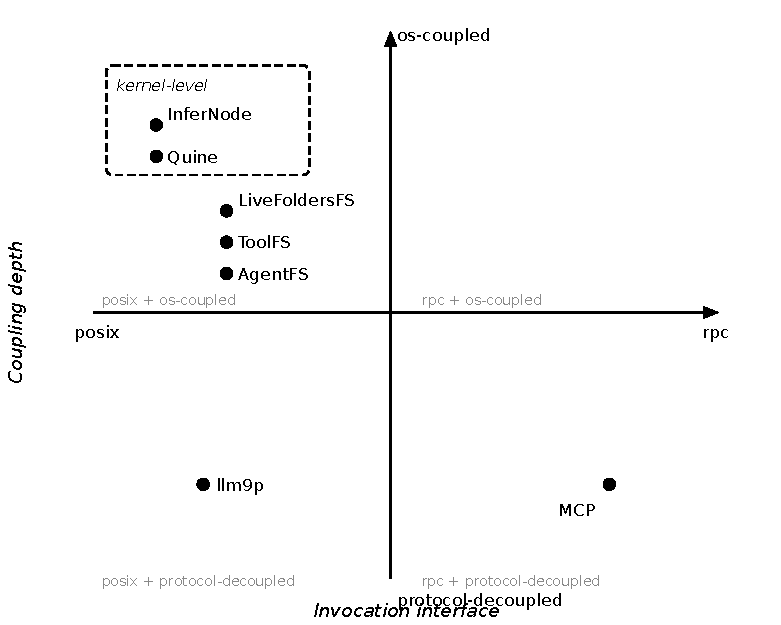
\includegraphics{figures/taxonomy.pdf}
\caption{Taxonomy of LLM tool integration systems.}
\end{figure}

\hypertarget{empirical-comparison}{%
\section{Empirical Comparison}\label{empirical-comparison}}

\hypertarget{methodology}{%
\subsection{Methodology}\label{methodology}}

We evaluate all seven systems against ten criteria drawn from
practitioner requirements for production tool-integration
infrastructure. Criteria were selected to cover the full lifecycle of
tool integration: authoring (setup complexity, stateful tools), runtime
(LLM compatibility, I/O expressiveness, security, observability,
hot-reload), and ecosystem (discoverability, composability, publishing).

\textbf{Evidence tiers.} We use three evidence levels, consistently
labeled throughout:

\begin{itemize}
\tightlist
\item
  \emph{T1 (live experiment)}: The system is installed, run, and tested
  against real tasks on the evaluation host (Claude Code, Linux
  x86\_64). Results are directly observed and reproducible via
  \texttt{bash\ research/run-all.sh}.
\item
  \emph{T2 (structured assessment)}: The system is assessed via code
  reading, install testing, and documentation review. Claims made in
  code or documentation are noted but not independently verified against
  running behavior.
\item
  \emph{T3 (paper-only)}: The system is assessed from its published
  description only. No implementation was available for direct
  examination.
\end{itemize}

\textbf{Rating scale.} ✓ (strong): the system clearly satisfies the
criterion. \textasciitilde{} (partial): the system partially satisfies
the criterion or satisfies it with significant caveats. ✗ (weak): the
system does not satisfy the criterion or satisfies it only with major
workarounds. --- (N/A): the criterion does not apply to this system's
architectural role.

T1 systems are LiveFoldersFS and MCP. T2 systems are ToolFS, AgentFS,
and llm9p. T3 systems are InferNode and Quine. All T1 experiments are
publicly available and reproducible from the repository root.

\hypertarget{results}{%
\subsection{Results}\label{results}}

\begin{longtable}[]{@{}
  >{\raggedright\arraybackslash}p{(\columnwidth - 14\tabcolsep) * \real{0.12}}
  >{\raggedright\arraybackslash}p{(\columnwidth - 14\tabcolsep) * \real{0.12}}
  >{\raggedright\arraybackslash}p{(\columnwidth - 14\tabcolsep) * \real{0.12}}
  >{\raggedright\arraybackslash}p{(\columnwidth - 14\tabcolsep) * \real{0.12}}
  >{\raggedright\arraybackslash}p{(\columnwidth - 14\tabcolsep) * \real{0.12}}
  >{\raggedright\arraybackslash}p{(\columnwidth - 14\tabcolsep) * \real{0.12}}
  >{\raggedright\arraybackslash}p{(\columnwidth - 14\tabcolsep) * \real{0.12}}
  >{\raggedright\arraybackslash}p{(\columnwidth - 14\tabcolsep) * \real{0.12}}@{}}
\toprule
Criterion & LiveFoldersFS (T1) & MCP (T1) & ToolFS (T2) & AgentFS (T2) &
llm9p (T2) & InferNode (T3) & Quine (T3) \\
\midrule
\endhead
01 Setup complexity & ✓ & \textasciitilde{} & \textasciitilde{} &
\textasciitilde{} & \textasciitilde{} & ✗ & \textasciitilde{} \\
02 LLM compatibility & \textasciitilde{} & \textasciitilde{} &
\textasciitilde{} & \textasciitilde{} & \textasciitilde{} &
\textasciitilde{} & \textasciitilde{} \\
03 Discoverability & ✓ & \textasciitilde{} & \textasciitilde{} & --- &
--- & \textasciitilde{} & \textasciitilde{} \\
04 I/O expressiveness & \textasciitilde{} & \textasciitilde{} &
\textasciitilde{} & \textasciitilde{} & \textasciitilde{} &
\textasciitilde{} & ✓ \\
05 Security & ✓ & ✓ & \textasciitilde{} & \textasciitilde{} & ✗ & ✓ &
\textasciitilde{} \\
06 Stateful tools & ✓ & \textasciitilde{} & ✓ & \textasciitilde{} &
\textasciitilde{} & \textasciitilde{} & \textasciitilde{} \\
07 Composability & ✓ & \textasciitilde{} & \textasciitilde{} & --- &
\textasciitilde{} & ✓ & ✓ \\
08 Observability & ✓ & ✓ & \textasciitilde{} & ✓ & ✗ & \textasciitilde{}
& \textasciitilde{} \\
09 Hot-reload & ✓ & ✗ & ✗ & --- & \textasciitilde{} & \textasciitilde{}
& \textasciitilde{} \\
10 Publishing & ✓ & \textasciitilde{} & \textasciitilde{} & --- & --- &
✗ & \textasciitilde{} \\
\bottomrule
\end{longtable}

\emph{Table 2: 7×10 comparison matrix. Rating key: ✓ strong \textbar{}
\textasciitilde{} partial \textbar{} ✗ weak \textbar{} --- N/A. Evidence
tiers: T1 = live experiment \textbar{} T2 = structured assessment
\textbar{} T3 = paper-only.}

\hypertarget{per-criterion-findings}{%
\subsection{Per-Criterion Findings}\label{per-criterion-findings}}

\textbf{01 Setup complexity.} This criterion measures how many lines of
new code an author must write to expose a simple tool (a
string-transformation endpoint). LiveFoldersFS achieves ✓ (strong) with
a 6-line \texttt{folder.yaml} declaration requiring no Python or Go.
MCP, ToolFS, AgentFS, llm9p, and Quine all rate \textasciitilde{}
(partial): they require more code (MCP's minimal server is 8 lines
before imports, with more needed for production), additional
dependencies, or non-trivial configuration. InferNode rates ✗ (weak):
its kernel-level integration requires the author to understand Inferno
namespace conventions and Limbo, a language with a narrow practitioner
base. The LiveFoldersFS advantage is structural --- YAML declarative
configuration collapses the authoring model to the minimum expressible
for simple tools, while handlers are shell one-liners.

\textbf{02 LLM compatibility.} All seven systems rate \textasciitilde{}
(partial) on this criterion. The reasons differ by quadrant. Os-coupled
posix systems (LiveFoldersFS, ToolFS, AgentFS, InferNode, Quine) require
the LLM agent to have shell or filesystem access --- which Claude Code
has, but API-only deployments typically do not. Protocol-decoupled
systems (MCP, llm9p) require the LLM client to implement the relevant
protocol --- MCP is widely implemented in major agent frameworks, but
llm9p's 9P-over-TCP interface has no native support in any major LLM
client as of this writing. No system achieves universal compatibility
without a compatibility shim.

\textbf{03 Discoverability.} How does an LLM learn what tools are
available and how to call them? LiveFoldersFS rates ✓ (strong) as of
v0.8.0: it now exposes both a human-readable \texttt{how\_to.md} and a
machine-readable \texttt{schema.json} generated from
\texttt{folder.yaml}. The \texttt{schema.json} mirrors MCP's
\texttt{list\_tools} format --- a JSON object with \texttt{name},
\texttt{description}, and an \texttt{endpoints} array where each entry
carries \texttt{name}, \texttt{kind}, and the full \texttt{input}
constraint block (\texttt{type}, \texttt{min\_length},
\texttt{max\_length}, \texttt{pattern}, \texttt{schema}). This makes the
tool surface parseable by MCP-aware clients and scripts without
requiring markdown parsing. MCP rates \textasciitilde{} (partial): its
\texttt{list\_tools} response is strong for clients that implement the
protocol, but there is no fallback for agents with only filesystem
access. ToolFS follows a file-listing approach similar to
LiveFoldersFS's \texttt{how\_to.md} but provides no machine-readable
schema file. AgentFS and llm9p rate --- (N/A): AgentFS is a storage
substrate with no tool-invocation interface to discover, and llm9p's
architectural inversion means there are no tools to discover in the
conventional sense. InferNode and Quine rate \textasciitilde{} based on
their published descriptions of namespace-based discovery.

\textbf{04 I/O expressiveness.} What data types can a tool consume and
produce? All systems handle plain text and JSON strings. LiveFoldersFS
rates \textasciitilde{} because it passes raw stdin to handlers ---
well-suited for multiline text and binary piping. v0.7.0 adds structural
constraints enforced before the handler runs: string endpoints can
declare \texttt{min\_length}, \texttt{max\_length}, and a regex
\texttt{pattern}; JSON endpoints can declare a \texttt{schema:} block
with \texttt{required} field lists and per-property type constraints
(\texttt{string}, \texttt{number}, \texttt{integer}, \texttt{boolean},
\texttt{array}, \texttt{object}, \texttt{null}). Violations produce a
structured \texttt{{[}ERROR:INVALID\_INPUT{]}} response without
executing any shell code. The remaining gap versus MCP is that
LiveFoldersFS constraints are opt-in per endpoint while MCP validation
is unconditional; additionally, MCP supports nested JSON Schema features
(e.g., \texttt{enum}, \texttt{oneOf}, \texttt{additionalProperties})
that LiveFoldersFS's subset does not yet implement. MCP rates
\textasciitilde{} for the same reason as before: structured JSON is
strong, but multiline text requires string escaping and binary data
requires base64 encoding. The notable outlier is Quine (✓), which
operates at the kernel level and can pass arbitrary byte streams through
Inferno's typed channels. InferNode similarly benefits from kernel-level
data access. No surveyed system simultaneously achieves type safety
(MCP's strength) and binary transparency (Quine's strength).

\textbf{05 Security.} This criterion reveals sharp divergence in the
survey. MCP rates ✓ (strong): input schemas are enforced before any
handler executes, rejecting malformed inputs before they reach
application code. InferNode rates ✓ at the kernel level, where namespace
isolation provides OS-enforced boundaries. LiveFoldersFS rates ✓
(strong) as of v0.11.0, achieving security through two complementary
layers. The first is opt-in structural input validation introduced in
v0.7.0: string endpoints can specify \texttt{min\_length},
\texttt{max\_length}, and a regex \texttt{pattern}; JSON endpoints can
specify a \texttt{schema:} block enforcing required fields and
per-property type constraints. The runtime rejects inputs that violate
any declared constraint before invoking any shell code, returning a
structured \texttt{{[}ERROR:INVALID\_INPUT{]}} response. For a tool
declaring
\texttt{input:\ \{type:\ json,\ schema:\ \{required:\ {[}query{]},\ properties:\ \{query:\ \{type:\ string\}\}\}\}},
passing \texttt{\{\}} yields
\texttt{{[}ERROR:INVALID\_INPUT{]}\ missing\ required\ field:\ \textquotesingle{}query\textquotesingle{}}
and passing \texttt{\{"query":\ 42\}} yields
\texttt{{[}ERROR:INVALID\_INPUT{]}\ field\ \textquotesingle{}query\textquotesingle{}\ expected\ type\ \textquotesingle{}string\textquotesingle{}}
--- both without executing the handler. The second layer is VFS-layer
process isolation introduced in v0.11.0: every handler on Linux executes
inside a sandbox comprising \texttt{PR\_SET\_NO\_NEW\_PRIVS} (preventing
privilege escalation), Landlock LSM filesystem access control
(configurable read/write path allowlists; \texttt{/usr}, \texttt{/lib},
\texttt{/etc/ssl/certs}, and \texttt{/tmp} are permitted by default),
seccomp-BPF network isolation (blocking \texttt{socket()} by default),
and configurable \texttt{RLIMIT\_NPROC}/\texttt{RLIMIT\_AS} resource
limits. Per-tool policy is declared in a \texttt{sandbox:} block in
\texttt{folder.yaml}; global enforcement is controlled by
\texttt{sandbox\_mode:\ strict\ \textbar{}\ warn\ \textbar{}\ disabled}
in \texttt{livefolders.yaml}. The default \texttt{warn} mode applies the
sandbox where the kernel supports it (Linux ≥ 5.13 for Landlock) and
logs a degradation warning on older kernels rather than refusing to run.
The remaining gap versus MCP is that input validation remains opt-in per
endpoint (a handler author must declare the schema), while MCP
validation is unconditional at the protocol layer. llm9p rates ✗ for a
distinct and more severe reason --- by default, it binds an
unauthenticated TCP port, making the tool surface accessible to any
process on the network. This is the worst security finding in the survey
and represents a deployment risk in multi-tenant or networked
environments. ToolFS and AgentFS rate \textasciitilde{} (partial);
notably, ToolFS's documentation claims WASM sandbox isolation, but code
inspection (T2) reveals this is implemented as \texttt{InMemorySandbox}
--- a stub with no actual isolation. The security claim in ToolFS's
documentation does not reflect the current implementation.

\textbf{06 Stateful tools.} How well does each system support tools that
maintain state across invocations? LiveFoldersFS and ToolFS both rate ✓
(strong). ToolFS uses in-process Go plugin state (fast, but lost on
restart). LiveFoldersFS v0.8.0 adds a \texttt{state\_file} field to
\texttt{FileSpec}: a tool author declares
\texttt{state\_file:\ /var/data/my-tool.db} in \texttt{folder.yaml}, and
the runtime passes
\texttt{LIVEFOLDERS\_STATE\_FILE=/var/data/my-tool.db} to the handler
while holding an exclusive POSIX advisory lock
(\texttt{flock(LOCK\_EX)}) for the duration of the call. This prevents
concurrent invocations from corrupting shared state without requiring
the handler author to manage locking. The lock is acquired before the
process starts and released on exit, making it transparent to shell
scripts and any executable handler. State is durable across restarts
because it lives in a user-specified file, not in process memory. MCP
rates \textasciitilde{} (partial): state lives in Python process memory
--- fast but ephemeral. InferNode and Quine rate \textasciitilde{} based
on published descriptions of kernel-level state management. No surveyed
system provides transactional consistency (e.g., ACID semantics) without
an embedded database; the advisory lock in LiveFoldersFS prevents races
but does not provide rollback.

\textbf{07 Composability.} This criterion measures how easily tool
outputs can be chained or combined. LiveFoldersFS, Quine, and InferNode
rate ✓ (strong). Quine and InferNode leverage Inferno's per-process
namespaces to compose tool environments hierarchically. LiveFoldersFS
v0.9.0 adds a \texttt{pipe:} field to \texttt{FileSpec}: an author
declares an ordered list of existing endpoint names, and the runtime
chains them --- the stdout of each stage becomes the stdin of the next,
within a single write invocation by the LLM. A \texttt{folder.yaml}
entry of \texttt{pipe:\ {[}fetch\_weather,\ format\_report{]}} means
\texttt{echo\ "London"\ \textgreater{}\ weather\_report} atomically
invokes both handlers in sequence and returns the final output, with no
intermediate reads required. Per-stage input schemas are validated
before each stage executes, and any stage error stops the pipeline
immediately with a structured \texttt{{[}ERROR:CODE{]}} response. MCP
rates \textasciitilde{} (partial): Python function composition is clean
within a single server, but cross-server tool chaining requires LLM
orchestration. ToolFS and llm9p also rate \textasciitilde{} with no
native pipeline mechanism. AgentFS rates --- (N/A) as a storage
substrate.

\textbf{08 Observability.} How well does the system support diagnosing
errors and monitoring tool execution? LiveFoldersFS, MCP, and AgentFS
all rate ✓ (strong). MCP converts Python exceptions to structured error
objects with type, message, and traceback. AgentFS is purpose-built as
an observability substrate, providing structured audit logs and
execution traces as first-class filesystem artifacts; however, 4 of 10
criteria rate --- (N/A) for AgentFS because it is a storage and
observation layer rather than a tool-invocation interface. LiveFoldersFS
rates ✓ as of v0.8.0: after every invocation, the runtime writes a
companion \texttt{\textless{}endpoint\textgreater{}.log} file alongside
the endpoint file. The log records \texttt{duration\_ms} and the full
\texttt{stderr} of the last run, making timing and diagnostics
immediately readable with \texttt{cat\ forecast.log} or any file-reading
operation. An LLM or monitoring script can observe execution duration
and check stderr without round-tripping through the tool itself. Error
returns continue to use the structured
\texttt{{[}ERROR:CODE{]}\ message} format with five machine-parseable
codes (\texttt{HANDLER}, \texttt{TIMEOUT}, \texttt{SPAWN},
\texttt{PROCESS}, \texttt{INVALID\_INPUT}) established in v0.6.0.
Together these provide two observability layers: structured error codes
in the response stream and a per-endpoint log file for post-hoc
inspection. llm9p rates ✗ (weak): its architectural inversion means
there is no clear place in its design for tool execution observability.
ToolFS rates \textasciitilde{} with no equivalent to structured traces
or timing.

\textbf{09 Hot-reload.} Can a tool author modify a handler and see the
change reflected without restarting or reconnecting? LiveFoldersFS rates
✓ (strong): an inotify watcher detects changes to \texttt{folder.yaml}
or handler scripts; updated handlers are visible within approximately
one second, with no agent reconnection required. MCP rates ✗ (weak):
modifying \texttt{server.py} requires killing the MCP server process,
restarting it, and waiting for Claude Code to complete the reconnect
handshake (approximately 1--3 seconds for Python startup plus protocol
negotiation). ToolFS also rates ✗ on hot-reload; its Go plugin
architecture requires recompilation. AgentFS rates --- as a storage
substrate. llm9p, InferNode, and Quine rate \textasciitilde{} based on
published descriptions suggesting partial support.

\textbf{10 Publishing.} How easy is it to distribute a tool for others
to install? LiveFoldersFS rates ✓ (strong): any GitHub repository
containing a \texttt{folder.yaml} is immediately installable with
\texttt{livefolders\ install\ github.com/you/repo}. There is no
registry, no package upload, and no configuration editing required. MCP
rates \textasciitilde{} (partial): options include npm/PyPI publication,
listing in community registries (no official registry exists as of this
writing), or sharing a repository URL for manual configuration. ToolFS,
AgentFS (as a storage layer), InferNode, and Quine rate
\textasciitilde{} or --- based on lack of any publishing infrastructure.
The publishing gap between LiveFoldersFS and the rest of the field is
the largest single-criterion gap in the matrix: only one surveyed system
treats tool distribution as a first-class design concern.

\hypertarget{worked-example-users-rest-api}{%
\subsection{Worked Example: Users REST
API}\label{worked-example-users-rest-api}}

To illustrate the authoring experience concretely, we implement a
minimal tool that fetches a list of users from a REST API and returns
formatted markdown. This is a representative task: a single external
HTTP call, structured data, markdown output.

\textbf{LiveFoldersFS implementation} (\texttt{folder.yaml}, 10 lines):

\begin{Shaded}
\begin{Highlighting}[]
\FunctionTok{name}\KeywordTok{:}\AttributeTok{ users}
\FunctionTok{description}\KeywordTok{:}\AttributeTok{ List users from the mock API.}
\FunctionTok{files}\KeywordTok{:}
\AttributeTok{  }\KeywordTok{{-}}\AttributeTok{ }\FunctionTok{name}\KeywordTok{:}\AttributeTok{ list}
\AttributeTok{    }\FunctionTok{type}\KeywordTok{:}\AttributeTok{ read\_invoke}
\FunctionTok{    handler}\KeywordTok{: }\CharTok{\textgreater{}{-}}
\NormalTok{      curl {-}s https://6a0b5d085aa893e1015a2d32.mockapi.io/users}
\NormalTok{      | jq {-}r \textquotesingle{}"\# Users\textbackslash{}n", (.[] | "\#\# \textbackslash{}(.name)\textbackslash{}nID: \textbackslash{}(.id)\textbackslash{}nCreated: \textbackslash{}(.createdAt)\textbackslash{}nAvatar: \textbackslash{}(.avatar)\textbackslash{}n")\textquotesingle{}}
\AttributeTok{  }\KeywordTok{{-}}\AttributeTok{ }\FunctionTok{name}\KeywordTok{:}\AttributeTok{ how\_to.md}
\AttributeTok{    }\FunctionTok{type}\KeywordTok{:}\AttributeTok{ readonly}
\end{Highlighting}
\end{Shaded}

\textbf{MCP implementation} (\texttt{server.py}, 18 lines):

\begin{Shaded}
\begin{Highlighting}[]
\ImportTok{import}\NormalTok{ httpx}
\ImportTok{from}\NormalTok{ mcp.server.fastmcp }\ImportTok{import}\NormalTok{ FastMCP}
\NormalTok{mcp }\OperatorTok{=}\NormalTok{ FastMCP(}\StringTok{"users"}\NormalTok{)}

\AttributeTok{@mcp.tool}\NormalTok{()}
\KeywordTok{def}\NormalTok{ list\_users() }\OperatorTok{{-}\textgreater{}} \BuiltInTok{str}\NormalTok{:}
    \CommentTok{"""Fetches all users from the JSONPlaceholder API."""}
\NormalTok{    response }\OperatorTok{=}\NormalTok{ httpx.get(}\StringTok{"https://jsonplaceholder.typicode.com/users"}\NormalTok{)}
\NormalTok{    response.raise\_for\_status()}
\NormalTok{    users }\OperatorTok{=}\NormalTok{ response.json()}
\NormalTok{    lines }\OperatorTok{=}\NormalTok{ [}\StringTok{"\# Users"}\NormalTok{, }\StringTok{""}\NormalTok{]}
    \ControlFlowTok{for}\NormalTok{ u }\KeywordTok{in}\NormalTok{ users:}
\NormalTok{        lines.append(}\SpecialStringTok{f"\#\# }\SpecialCharTok{\{u}\NormalTok{[}\StringTok{\textquotesingle{}name\textquotesingle{}}\NormalTok{]}\SpecialCharTok{\}}\SpecialStringTok{"}\NormalTok{)}
\NormalTok{        lines.append(}\SpecialStringTok{f"ID: }\SpecialCharTok{\{u}\NormalTok{[}\StringTok{\textquotesingle{}id\textquotesingle{}}\NormalTok{]}\SpecialCharTok{\}}\SpecialStringTok{"}\NormalTok{)}
\NormalTok{        lines.append(}\SpecialStringTok{f"Email: }\SpecialCharTok{\{u}\NormalTok{[}\StringTok{\textquotesingle{}email\textquotesingle{}}\NormalTok{]}\SpecialCharTok{\}}\SpecialStringTok{"}\NormalTok{)}
\NormalTok{        lines.append(}\StringTok{""}\NormalTok{)}
    \ControlFlowTok{return} \StringTok{"}\CharTok{\textbackslash{}n}\StringTok{"}\NormalTok{.join(lines)}

\ControlFlowTok{if} \VariableTok{\_\_name\_\_} \OperatorTok{==} \StringTok{"\_\_main\_\_"}\NormalTok{:}
\NormalTok{    mcp.run()}
\end{Highlighting}
\end{Shaded}

The line count difference (10 vs 18) reflects the YAML declaration model
versus an explicit Python server. Note that the two implementations use
different upstream APIs (mockapi.io vs jsonplaceholder.typicode.com)
because the worked example was developed independently for each system;
the functional structure is equivalent.

From Claude Code's perspective, the two implementations produce distinct
interaction patterns. With LiveFoldersFS, Claude reads the result with a
file read operation: \texttt{cat\ /mnt/livefolders/users/list}. The tool
output arrives as plain text in the file read response ---
indistinguishable from reading any other file. With MCP, Claude invokes
a structured tool call:
\texttt{\{"method":\ "tools/call",\ "params":\ \{"name":\ "list\_users",\ "arguments":\ \{\}\}\}},
receiving a structured response with \texttt{content} and
\texttt{isError} fields. Both approaches are legible to Claude Code,
consistent with the \textasciitilde{} (partial) LLM compatibility rating
for both systems.

Extending this example to other systems in the survey is instructive.
ToolFS would require the author to write a Go plugin compiled to a
shared library --- significantly more infrastructure than either example
above. llm9p does not support tool invocation in this direction at all:
its architecture inverts the relationship, serving the LLM's context as
a filesystem rather than serving external tools to an LLM.

\hypertarget{related-work}{%
\section{Related Work}\label{related-work}}

\hypertarget{llm-tool-use-foundations}{%
\subsection{LLM Tool Use Foundations}\label{llm-tool-use-foundations}}

The use of LLMs as tool-calling agents has been studied extensively.
ReAct (Yao et al. 2023) established the interleaved reasoning-and-action
paradigm, showing that LLMs can alternate between generating thoughts
and executing actions (tool calls) to solve complex tasks. Gorilla
(Patil et al. 2024) demonstrated that LLMs can be fine-tuned to generate
accurate API calls, surfacing the challenge of tool hallucination and
the importance of retrieval-augmented tool documentation. ToolBench (Qin
et al. 2024) introduced a large-scale benchmark of real-world REST APIs
with an associated training dataset, establishing evaluation
infrastructure for tool-use capabilities.

These works study \emph{which} tools LLMs can effectively use and
\emph{how well} they can select and invoke them. Our work is orthogonal:
we study how the \emph{interface layer} between the LLM and tools is
architected. The tool-use capability studies presuppose some integration
mechanism; we examine the design space of those mechanisms
systematically.

\hypertarget{the-everything-is-a-file-lineage}{%
\subsection{The ``Everything is a File''
Lineage}\label{the-everything-is-a-file-lineage}}

The principle that resources should be represented as files is a
foundational design philosophy of Unix, articulated most completely in
Plan 9 from Bell Labs (Pike et al. 1990). Plan 9 extended the file
abstraction universally --- network connections, process state, and
device interfaces are all files --- enabling a uniform interface for
composition and access control. The Linux Filesystem in Userspace (FUSE)
brought user-space virtual filesystems to Linux, allowing arbitrary
software to implement the filesystem interface without kernel
privileges.

In 2024--2026, multiple teams independently applied this lineage to LLM
agent tool integration. ToolFS (IceWhaleTech 2024) exposes Go plugins as
a FUSE filesystem. AgentFS (Turso 2024) builds a shared agent storage
substrate on FUSE with observability as a first-class concern. llm9p
(NERVsystems 2025b) revisits the Plan 9 philosophy directly, using the
9P protocol to serve an LLM's context as a filesystem --- though it
inverts the typical direction of tool integration. InferNode
(NERVsystems 2025a) goes further, embedding LLM inference as a kernel
service in a Plan 9-derived operating system. Quine (Anonymous 2025)
applies Inferno's per-process namespace model to give each agent a
private, composable tool environment. DMI (Wang, Li, and Chen 2025)
extends filesystem metaphors to GUI navigation for agents. LiveFoldersFS
(Loterio 2025) targets the authoring experience, making tool creation a
matter of YAML configuration backed by shell handlers.

The independent convergence of multiple teams on filesystem abstractions
for LLM tool integration --- without coordination and across different
implementation languages and OS layers --- is the empirical signal that
motivates our taxonomy. When practitioners independently rediscover the
same abstraction, it suggests the abstraction offers genuine
affordances. Our survey is the first to document and explain this
convergence systematically.

\hypertarget{protocol-based-integration}{%
\subsection{Protocol-Based
Integration}\label{protocol-based-integration}}

MCP (Anthropic 2024) defines an open standard for tool integration via
JSON-RPC over stdio or HTTP. It specifies tool discovery
(\texttt{list\_tools}), invocation (\texttt{tools/call}), and error
handling in a protocol-agnostic way. MCP was donated to the Linux
Foundation in December 2025, signaling institutional commitment to its
longevity as an open standard. OpenAI's function calling and LangChain's
tool abstractions operate at the SDK layer over conceptually similar RPC
models, though they are not interoperable with MCP at the protocol
level.

Our empirical comparison is the first systematic evaluation of MCP
against filesystem-native alternatives across a common criterion set.
Prior published comparisons are either promotional (originating from
system authors) or informal (blog posts, developer discussions). The
structured assessment methodology we apply, with explicit evidence
tiers, provides a more reliable basis for comparison.

LSFS (Shi et al. 2025) represents a direction distinct from both
paradigms: rather than LLMs calling tools through a filesystem
interface, LSFS makes the filesystem itself semantically aware,
answering natural-language queries about file content and structure.
This LLM-enhanced filesystem paradigm addresses a different user need
(human file management augmented by LLM) and is not directly comparable
to the tool-integration systems in our survey.

\hypertarget{design-principles-and-future-directions}{%
\section{Design Principles and Future
Directions}\label{design-principles-and-future-directions}}

Three design principles emerge from the empirical evidence.

\textbf{Principle 1: Coupling depth determines ergonomics ceiling.}

Os-coupled systems inherit decades of POSIX tooling. Any CLI utility,
\texttt{curl} command, shell pipeline, or script in any language is
immediately usable as a tool handler without modification. This is a
structural advantage --- it cannot be replicated by protocol-decoupled
systems without adding an OS-level layer. The worked example illustrates
this concretely: the LiveFoldersFS \texttt{folder.yaml} (10 lines)
requires no Python, no imports, no server lifecycle management, and no
protocol knowledge. The MCP \texttt{server.py} (18 lines) requires all
of these. The absolute line-count difference is modest for a simple
case; the gap grows with tool complexity, because every MCP tool must
navigate the server framework, while every LiveFoldersFS tool is
independently a shell command.

The tradeoff is portability. Os-coupled systems require the agent to
have shell and filesystem access on the host where tools are mounted. In
cloud-hosted agent deployments where the LLM accesses tools over a
network, os-coupling requires either a local agent proxy or explicit
infrastructure to bridge the network boundary. Protocol-decoupled
systems like MCP operate naturally over HTTP and can expose tools
running on remote hosts to agents anywhere.

\textbf{Principle 2: Invocation interface determines safety floor.}

RPC systems enforce input schemas before any handler executes. A poorly
written MCP tool automatically rejects inputs that do not match its
declared parameter schema; the validation happens at the protocol layer,
not the application layer. The posix invocation model historically
concentrated security responsibility entirely on the individual handler
author. LiveFoldersFS v0.7.0 substantially narrows this gap through
richer opt-in structural validation: declaring
\texttt{input:\ \{type:\ string,\ min\_length:\ 1,\ max\_length:\ 500,\ pattern:\ "\^{}\textbackslash{}\textbackslash{}w+\$"\}}
enforces all three constraints before the handler runs; declaring
\texttt{input:\ \{type:\ json,\ schema:\ \{required:\ {[}query{]},\ properties:\ \{query:\ \{type:\ string\}\}\}\}}
enforces required fields and property types. All violations produce
\texttt{{[}ERROR:INVALID\_INPUT{]}} responses without executing shell
code. This brings the posix authoring model meaningfully closer to the
safety guarantees of RPC systems for well-authored tools. The remaining
structural gap is twofold: MCP validation is unconditional (every tool
is validated, even if the author writes no schema), while LiveFoldersFS
validation requires explicit per-endpoint opt-in; and MCP supports the
full JSON Schema vocabulary, while LiveFoldersFS's \texttt{schema:} key
currently implements a subset (required, properties with type
constraints) sufficient for the most common validation patterns.

Our survey found the most severe security failure in the
posix-invocation quadrant: llm9p's unauthenticated TCP port is
accessible to any network process, a vulnerability that does not exist
in MCP's stdio-based transport. The correlation between invocation
interface and security rating is not perfect (AgentFS rates
\textasciitilde{} despite posix invocation, InferNode rates ✓ with posix
invocation through kernel namespace isolation), but the tendency is real
and systematic.

\textbf{Principle 3: Publishing model is underexplored.}

Only LiveFoldersFS treats tool distribution as a first-class design
concern. A single command ---
\texttt{livefolders\ install\ github.com/you/repo} --- installs any
\texttt{folder.yaml} from any GitHub repository, with no registry
registration, no package upload, and no configuration editing by the end
user. All other surveyed systems require either manual configuration
(MCP: editing \texttt{claude\_desktop\_config.json}; ToolFS: compiling
and placing a Go shared library), registration in a community registry
(with no official MCP registry as of this writing), or are not designed
for distribution at all (AgentFS, InferNode, Quine). As the LLM tool
ecosystem matures, discoverability and install friction will determine
whether tool ecosystems grow organically or remain fragmented. Systems
that treat publishing as an afterthought will face an adoption ceiling
that ergonomics advantages cannot overcome.

\textbf{Future directions.} Four technical directions appear most
promising given the observed tradeoffs.

\emph{VFS-layer sandboxing} has been implemented in LiveFoldersFS
v0.11.0, realizing the combination of os-coupling's ergonomic advantages
with rpc-coupling's process isolation guarantees. Handlers on Linux now
execute inside a sandbox comprising Landlock LSM filesystem access
control, seccomp-BPF network isolation,
\texttt{PR\_SET\_NO\_NEW\_PRIVS}, and configurable
\texttt{RLIMIT\_NPROC}/\texttt{RLIMIT\_AS} resource limits --- all
applied transparently before the handler process starts, without
requiring handler authors to change their shell scripts. ToolFS gestures
at this direction with its WASM sandbox design, but code inspection (T2)
reveals the implementation is a stub; LiveFoldersFS v0.11.0 closes the
gap with a verified, running implementation. The remaining frontier is
platform parity: the macOS implementation exists but provides weaker
guarantees than the Linux path, and Windows WSL environments are
unsupported. A complementary open question is whether sandboxing can be
made unconditional by default --- matching MCP's validation model ---
rather than requiring opt-in via a \texttt{sandbox:} block per tool.

\emph{Hybrid architectures} would use a filesystem view as the authoring
and invocation interface for LLMs while delegating to MCP servers as the
actual handler execution layer. Tool authors would write MCP servers as
today; a filesystem bridge would expose those servers as files to
shell-capable agents, providing hot-reload and shell ergonomics at the
tool-author layer while preserving schema validation at the transport
layer.

\emph{Richer schema enforcement} has been implemented in LiveFoldersFS
v0.7.0: string endpoints now support \texttt{min\_length},
\texttt{max\_length}, and \texttt{pattern} (regex) constraints; JSON
endpoints support a \texttt{schema:} block with \texttt{required} field
lists and \texttt{properties{[}*{]}.type} checks. These constraints are
enforced before any handler executes and surfaced inline in
auto-generated \texttt{how\_to.md}. The remaining frontier is full JSON
Schema support: \texttt{enum}, \texttt{oneOf}, \texttt{anyOf},
\texttt{additionalProperties}, \texttt{minimum}/\texttt{maximum} for
numbers, and nested object schemas are not yet implemented. A future
extension could delegate to the \texttt{jsonschema} crate for full
specification compliance.

\emph{Machine-readable schemas, stateful locking, execution tracing, and
declarative pipelines} have been implemented in LiveFoldersFS
v0.8.0--v0.9.0. A \texttt{schema.json} virtual file mirrors MCP's
\texttt{list\_tools} format, making the tool surface parseable by any
MCP-aware client alongside the human-readable \texttt{how\_to.md}. The
\texttt{state\_file} manifest field allows endpoints to declare a
persistent state path; the runtime acquires an exclusive POSIX advisory
lock (\texttt{flock(LOCK\_EX)}) before spawning the handler and passes
the path as \texttt{LIVEFOLDERS\_STATE\_FILE}, preventing concurrent
corruption without handler-side coordination. Finally, each invokable
endpoint now exposes a companion
\texttt{\textless{}endpoint\textgreater{}.log} file recording
\texttt{duration\_ms} and \texttt{stderr} from the last call, giving
agents and monitoring scripts post-hoc observability over timing and
diagnostics without round-tripping through the tool. These additions
bring LiveFoldersFS to ✓ on criteria 03, 06, and 08. v0.9.0 further adds
a \texttt{pipe:} field for declarative multi-stage chaining (criterion
07 ✓): an ordered list of endpoint names whose stdout/stdin are chained
within a single LLM write, with per-stage schema validation and
structured error propagation on stage failure.

\emph{Cross-platform FUSE} would extend os-coupled approaches to macOS
(where FUSE is less mature following the osxfuse/macFUSE fragmentation)
and Windows WSL environments. Current os-coupled systems are effectively
Linux-only in practice, limiting their addressable deployment surface.

\hypertarget{conclusion}{%
\section{Conclusion}\label{conclusion}}

LLM tool integration has produced a fragmented landscape of approaches,
each developed with implicit architectural assumptions and without
systematic comparison. We contributed a two-axis taxonomy organizing
seven systems along coupling depth (os-coupled vs.~protocol-decoupled)
and invocation interface (posix vs.~rpc), an empirical evaluation across
ten criteria using three evidence tiers, and three design principles
derived from the observed tradeoffs.

The central finding is that coupling depth and invocation interface are
the two dimensions that most explain system behavior --- and they trade
off against each other. Os-coupled systems (LiveFoldersFS, ToolFS,
AgentFS, InferNode, Quine) win on ergonomics, authoring speed,
hot-reload, and publishing; protocol-decoupled systems (MCP) win on
portability and unconditional schema enforcement. The gap is narrowing:
LiveFoldersFS v0.6.0 introduced opt-in per-endpoint input validation and
a structured \texttt{{[}ERROR:CODE{]}} error format; v0.7.0 extends this
to structural constraints --- string endpoints support
\texttt{min\_length}, \texttt{max\_length}, and regex \texttt{pattern};
JSON endpoints support a \texttt{schema:} sub-key with required-field
and property-type enforcement; v0.8.0 adds machine-readable
\texttt{schema.json} discovery (criterion 03 ✓), durable stateful
locking via \texttt{state\_file} + \texttt{flock} (criterion 06 ✓), and
per-invocation \texttt{.log} files with timing and stderr (criterion 08
✓); v0.9.0 adds declarative \texttt{pipe:} multi-stage chaining
(criterion 07 ✓), making LiveFoldersFS the only non-Inferno system to
achieve ✓ on composability; v0.11.0 implements opt-in VFS-layer
sandboxing via Landlock and seccomp-BPF (criterion 05 ✓). No current
system fully optimizes both dimensions simultaneously across all
criteria. The independent convergence of multiple teams on filesystem
abstractions for LLM tool integration validates the abstraction's
practical appeal; the remaining safety gap relative to protocol-based
systems explains why protocol approaches have gained institutional
traction.

The most striking finding from our Tier 2 assessment is the gap between
claimed and implemented behavior: ToolFS's WASM sandbox is a stub, not a
functioning isolation mechanism; llm9p's unauthenticated TCP transport
creates network-accessible tool surfaces. Practitioners evaluating these
systems should treat published claims about security properties as
hypotheses pending independent verification.

Future systems that resolve the coupling-versus-safety tension ---
through VFS-layer sandboxing, hybrid architectures, or schema inference
--- represent the most promising direction for the field. All
experiments underlying this evaluation are reproducible: code at the
LiveFoldersFS repository and \texttt{bash\ research/run-all.sh} from the
repository root.

\hypertarget{references}{%
\section*{References}\label{references}}
\addcontentsline{toc}{section}{References}

\hypertarget{refs}{}
\begin{CSLReferences}{1}{0}
\leavevmode\vadjust pre{\hypertarget{ref-quine2025}{}}%
Anonymous. 2025. {``Quine: Realizing {LLM} Agents as Native {POSIX}
Processes.''} \emph{arXiv Preprint arXiv:2603.18030}.
\url{https://arxiv.org/abs/2603.18030}.

\leavevmode\vadjust pre{\hypertarget{ref-mcp2024}{}}%
Anthropic. 2024. {``Model Context Protocol Specification.''}
\url{https://modelcontextprotocol.io/specification/2025-11-25}.

\leavevmode\vadjust pre{\hypertarget{ref-toolfs2024}{}}%
IceWhaleTech. 2024. {``{ToolFS}: A Virtual Filesystem for {LLM}
Agents.''} \url{https://github.com/IceWhaleTech/toolfs}.

\leavevmode\vadjust pre{\hypertarget{ref-livefolders2025}{}}%
Loterio, Natan. 2025. {``{LiveFoldersFS}: Expose Any Tool to an {LLM} as
Plain Files.''} \url{https://github.com/natanloterio/LiveFolders}.

\leavevmode\vadjust pre{\hypertarget{ref-infernode2025}{}}%
NERVsystems. 2025a. {``{InferNode}: Namespace-Based Alternative to {MCP}
Servers.''} \url{https://github.com/NERVsystems/infernode}.

\leavevmode\vadjust pre{\hypertarget{ref-llm9p2025}{}}%
---------. 2025b. {``{llm9p}: {LLM} as a Plan 9 File System.''}
\url{https://github.com/NERVsystems/llm9p}.

\leavevmode\vadjust pre{\hypertarget{ref-patil2023gorilla}{}}%
Patil, Shishir G., Tianjun Zhang, Xin Wang, and Joseph E. Gonzalez.
2024. {``Gorilla: Large Language Model Connected with Massive {APIs}.''}
In \emph{Advances in Neural Information Processing Systems}.
\url{https://arxiv.org/abs/2305.15334}.

\leavevmode\vadjust pre{\hypertarget{ref-pike1990plan9}{}}%
Pike, Rob, Dave Presotto, Ken Thompson, and Howard Trickey. 1990.
{``Plan 9 from {Bell Labs}.''} In \emph{USENIX Summer Conference}.

\leavevmode\vadjust pre{\hypertarget{ref-qin2023toolllm}{}}%
Qin, Yujia, Shengding Liang, Yining Ye, Kunlun Zhu, Lan Yan, Yaxi Lu,
Yankai Lin, et al. 2024. {``{ToolLLM}: Facilitating Large Language
Models to Master 16000+ Real-World {APIs}.''} In \emph{International
Conference on Learning Representations}.
\url{https://arxiv.org/abs/2307.16789}.

\leavevmode\vadjust pre{\hypertarget{ref-shi2024lsfs}{}}%
Shi, Zeru, Kai Ge, Yingqing Li, Zhen Xi, Wenyue Zhang, Zhu Xu, Juntao
Gao, et al. 2025. {``From Commands to Prompts: {LLM}-Based Semantic File
System for {AIOS}.''} In \emph{International Conference on Learning
Representations}. \url{https://arxiv.org/abs/2410.11843}.

\leavevmode\vadjust pre{\hypertarget{ref-agentfs2024}{}}%
Turso. 2024. {``{AgentFS}: The Missing Abstraction for {AI} Agents.''}
\url{https://github.com/tursodatabase/agentfs}.

\leavevmode\vadjust pre{\hypertarget{ref-wang2025dmi}{}}%
Wang, Yuan, Mingyu Li, and Haibo Chen. 2025. {``From Imperative to
Declarative: Towards {LLM}-Friendly {OS} Interfaces for Boosted
Computer-Use Agents.''} \emph{arXiv Preprint arXiv:2510.04607}.
\url{https://arxiv.org/abs/2510.04607}.

\leavevmode\vadjust pre{\hypertarget{ref-yao2023react}{}}%
Yao, Shunyu, Jeffrey Zhao, Dian Yu, Nan Du, Irina Shafran, Karthik
Narasimhan, and Yuan Cao. 2023. {``{ReAct}: Synergizing Reasoning and
Acting in Language Models.''} In \emph{International Conference on
Learning Representations}. \url{https://arxiv.org/abs/2210.03629}.

\end{CSLReferences}

\end{document}
